\section{Casimir energy of the Standard Model on a three-torus}\label{rep:casimir}

The Standard Model supplies the negative energy of a turning point when its fermions are antiperiodic.
With all three cycles of a cubic torus antiperiodic, its signed Casimir weight is $\NC=+25.515$, whereas periodic fermions give $-30$ (Sec.~\ref{rA:spin}). %
This chapter derives the image sum for twisted free fields from the mode sum (Sec.~\ref{rA:imagesum}), evaluates the lattice sums by an Ewald split (Sec.~\ref{rA:ewald}), assembles the Standard Model weights for every spin structure (Sec.~\ref{rA:spin}), and examines flat holonomies, 't~Hooft flux and the corrections to the field content (Secs.~\ref{rA:holonomy}--\ref{rA:content-corr}).
The energy of the constant modes, which does not depend on the shape and is a fraction $\fzm=0.30$ of the free Casimir energy at the cube, is the subject of Sec.~\ref{rep:zeromodes}, and the turning point that follows, at $\Lb=722\,\MPbar^{-1}$, that of Sec.~\ref{rep:turning}. %

\subsection{Vacuum energy of twisted free fields: the image sum}
\label{rA:imagesum}

\paragraph{Modes.}
On the torus with metric $h_{ij}=L^2G_{ij}$ and coordinates of unit period, a free massless field whose value changes by the phase $e^{2\pi i\vartheta_j}$ around the $j$th cycle has comoving wave vectors $\bm k=2\pi(\bm n+\bm\vartheta)$ with $\bm n\in\mathbb Z^3$.
Its physical frequencies are
\begin{equation}
\omega_{\bm n}=\frac{2\pi}{L}\Big[(\bm n+\bm\vartheta)^{\mathsf T}G^{-1}(\bm n+\bm\vartheta)\Big]^{1/2}.
\label{eq:rA-modes}
\end{equation}
Antiperiodic fermions have $\vartheta_j=\tfrac12$ on the antiperiodic cycles, and a flat gauge holonomy adds the charge times the holonomy phase to $\bm\vartheta$.

\paragraph{From modes to images.}
For one real bosonic degree of freedom the zero-point energy is $E_1=\tfrac12\sum_{\bm n}\omega_{\bm n}$.
Poisson summation, $\sum_{\bm n}f(\bm n+\bm\vartheta)=\sum_{\bm m}\hat f(\bm m)\,e^{2\pi i\bm m\cdot\bm\vartheta}$ with $\hat f(\bm m)=\int d^3\kappa\,f(\bm\kappa)e^{-2\pi i\bm m\cdot\bm\kappa}$, turns the mode sum into a sum over images.
For $f(\bm\kappa)=\tfrac12\omega(\bm\kappa)$ we change variables to the physical wave vector $\bm q=2\pi G^{-1/2}\bm\kappa/L$, whose Jacobian is $d^3\kappa=(L/2\pi)^3d^3q$ because $\det G=1$, and find
\begin{equation}
\hat f(\bm m)=L^3\int\frac{d^3q}{(2\pi)^3}\,\tfrac12|\bm q|\,e^{-i\bm q\cdot\bm x_{\bm m}},\qquad \bm x_{\bm m}=LG^{1/2}\bm m ,
\end{equation}
where $|\bm x_{\bm m}|^2=L^2\,\bm m^{\mathsf T}G\bm m$ is the squared physical length of the closed geodesic in the class $\bm m$.
The Fourier transform of $|\bm q|$ in three dimensions is, away from the origin,
\begin{equation}
\int\frac{d^3q}{(2\pi)^3}\,|\bm q|\,e^{i\bm q\cdot\bm x}=\frac{2}{\pi^{3/2}}\frac{\Gamma(2)}{\Gamma(-\tfrac12)}\frac{1}{|\bm x|^4}=-\frac{1}{\pi^2|\bm x|^4}.
\end{equation}
The term $\bm m=0$ is the energy of the same field in infinite space; it is proportional to the volume and renormalizes the cosmological constant.
The images $\bm m\neq0$ give the finite, regularization-independent part,
\begin{equation}
E_1=-\frac{1}{2\pi^2L}\sum_{\bm m\neq0}\frac{\cos(2\pi\bm\vartheta\cdot\bm m)}{(\bm m^{\mathsf T}G\bm m)^2},
\label{eq:rA-E1}
\end{equation}
after pairing $\bm m$ with $-\bm m$.
A Maxwell field has two polarizations, a Weyl fermion two helicity states with the opposite sign of the zero-point energy, and a real scalar one degree of freedom.

\paragraph{The image sum.}
Summing over fields, the vacuum energy of free massless fields with flat twists $\bm\vartheta_f$ is therefore the image sum~\cite{DeWitt:1979dd,Banach:1979iy,Bellucci:2009jr}
\begin{equation}
\begin{aligned}
E_C&=-\frac{1}{\pi^2L}\sum_{\bm n\neq0}\frac{w_{\bm n}}{(\bm n^{\mathsf T}G\bm n)^2},\\
w_{\bm n}&=\sum_fd_fs_f\cos(2\pi\bm\vartheta_f\cdot\bm n),
\end{aligned}
\label{eq:rA-imagesum}
\end{equation}
with $s_f=+1$ for bosons and $-1$ for fermions, and $d_f=1$ for a Maxwell field, a Weyl fermion or the static graviton and $\tfrac12$ for a real scalar.
Each image $\bm n$ contributes with the weight $w_{\bm n}$, the signed number of degrees of freedom that return to themselves around the closed geodesic $\bm n$.
Untwisted bosons give negative energy.
Periodic fermions ($\bm\vartheta=0$) therefore raise the energy, while antiperiodic fermions lower it~\cite{Arkani-Hamed:2007ryu,Ibanez:2017kvh}, because their images with odd $\sum_jn_j$ change sign; flat gauge holonomies twist charged fields in the same way.
We write $Z_s(G)=\sum'_{\bm n}(\bm n^{\mathsf T}G\bm n)^{-s}$ and $Z_s(G,\bm\vartheta)=\sum'_{\bm n}\cos(2\pi\bm\vartheta\cdot\bm n)(\bm n^{\mathsf T}G\bm n)^{-s}$, so that
\begin{equation}
E_C=-\frac{Z_{\rm eff}(G)}{\pi^2L},\qquad Z_{\rm eff}(G)=\sum_fd_fs_f\,Z_2(G,\bm\vartheta_f).
\label{eq:rA-Zeff}
\end{equation}

\subsection{Lattice constants of the cube}
\label{rA:lattice}

At the cube we write
\begin{equation}
\rho_C=\frac{E_C}{L^3}=-\frac{\NC\rAgam}{L^4},\qquad \rAgam=\frac{Z_2(\rAone)}{\pi^2}=1.6750738,\qquad \NC=\frac{1}{Z_2(\rAone)}\sum_{\bm n\neq0}\frac{w_{\bm n}}{|\bm n|^4},
\label{eq:rA-NC}
\end{equation} %
so that one periodic Maxwell field has $\NC=1$, and the Casimir coefficient of the torus is $C=\NC\rAgam=Z_{\rm eff}(\rAone)/\pi^2$, with $E_C=-C/L$.
For a periodic real scalar this is the familiar $E_C=-\rAgam/(2L)=-0.8375/L$.

On a single circle of length $L$ an antiperiodic field has the image weights $(-1)^n$, and
\begin{equation}
\sum_{n\geq1}\frac{(-1)^n}{n^4}=-\big(1-2^{-3}\big)\zeta(4),
\end{equation}
so an antiperiodic fermion contributes $7/8$ of the periodic magnitude with the opposite sign. %
On the cubic three-torus with all three cycles antiperiodic (AAA) the alternating lattice sum is much weaker:
\begin{equation}
Z_2\big(\rAone,(\tfrac12,\tfrac12,\tfrac12)\big)=\sum_{\bm n\neq0}\frac{(-1)^{n_1+n_2+n_3}}{|\bm n|^4}=-3.8631638, %
\label{eq:rA-aaa-sum}
\end{equation}
so an AAA Weyl fermion contributes $+3.8631638/16.5323160=+0.233673$ to $\NC$, while a periodic one contributes $-1$. %
The reason is a near cancellation between shells.
Images with even $n_1+n_2+n_3$ form the face-centered sublattice and contribute $Z_{\rm even}=6.3346$, and the odd images contribute $Z_{\rm odd}=10.1977$; the alternating sum is their difference. %
The six nearest images, $|\bm n|=1$, are odd and dominate, while the twelve next ones, $|\bm n|^2=2$, are even and cancel half of them.

\subsection{Ewald evaluation of the lattice sums}
\label{rA:ewald}

The sums of Eq.~\eqref{eq:rA-imagesum} converge slowly, and their shape derivatives more slowly still.
We evaluate $Z_2(G,\bm\vartheta)$ by an Ewald split.
With $Q_{\bm n}=\bm n^{\mathsf T}G\bm n$ we write $Q^{-2}=\int_0^\infty t\,e^{-tQ}\,dt$ and split the integral at $t=\pi$.
The upper part is elementary, $\int_\pi^\infty t\,e^{-tQ}dt=(1+\pi Q)e^{-\pi Q}/Q^2$.
In the lower part we complete the sum with the term $\bm n=0$, which contributes $\int_0^\pi t\,dt=\pi^2/2$ and is subtracted again, and apply Poisson summation to the Gaussian,
\begin{equation}
\sum_{\bm n}\cos(2\pi\bm\vartheta\cdot\bm n)\,e^{-tQ_{\bm n}}=\Big(\frac\pi t\Big)^{3/2}\frac{1}{\sqrt{\det G}}\sum_{\bm m}e^{-\pi^2P_{\bm m}/t},\qquad P_{\bm m}=(\bm m-\bm\vartheta)^{\mathsf T}G^{-1}(\bm m-\bm\vartheta).
\end{equation}
For $P_{\bm m}>0$ the substitution $t=\pi^2P_{\bm m}/x$ gives $\int_0^\pi t\,(\pi/t)^{3/2}e^{-\pi^2P/t}dt=\pi^{5/2}\sqrt P\,\Gamma(-\tfrac12,\pi P)$, and for $P_{\bm m}=0$, which occurs only for integer $\bm\vartheta$, the integral is $\pi^{3/2}\int_0^\pi t^{-1/2}dt=2\pi^2$.
Altogether
\begin{equation}
\begin{aligned}
Z_2={}&\sum_{\bm n\neq0}\cos(2\pi\bm\vartheta\cdot\bm n)\frac{(1+\pi Q_{\bm n})e^{-\pi Q_{\bm n}}}{Q_{\bm n}^2}-\frac{\pi^2}{2}\\
&+\frac{\pi^2}{\sqrt{\det G}}\Big[\sum_{P_{\bm m}>0}\sqrt{\pi P_{\bm m}}\,\Gamma(-\tfrac12,\pi P_{\bm m})+2\,\delta_{\bm\vartheta\in\mathbb Z^3}\Big],
\end{aligned}
\label{eq:rA-ewald}
\end{equation}
with $\Gamma(-\tfrac12,x)=2x^{-1/2}e^{-x}-2\sqrt\pi\,{\rm erfc}\sqrt x$.
Both sums now converge like Gaussians.
At the cube this gives $Z_2(\rAone,0)=16.5323159598$ and $Z_2(\rAone,(\tfrac12,\tfrac12,\tfrac12))=-3.8631638072$; a direct sum of the alternating series over $|n_i|\leq60$ agrees to $10^{-8}$. %
A separate implementation with $|n_i|,|m_i|\leq7$ reproduces both values to all printed digits. %
The same code, with derivatives of Eq.~\eqref{eq:rA-ewald} along the shape geodesics, gives the shape Hessians below and the shape forces of the nonlinear evolution in Sec.~\ref{rep:quantum-shape}.

\subsection{Spin structures}
\label{rA:spin}

At the turning point all Standard Model masses are negligible (Sec.~\ref{rA:scope}).
In the units of Eq.~\eqref{eq:rA-imagesum} the content of Sec.~\ref{rA:content} has $B=12+2+1=15$ for the gauge vectors, the Higgs doublet and the static graviton, and $F=45$ for the Weyl fermions. %
For the Standard Model plus the static graviton, $Z_{\rm eff}=15Z_2(G,0)-45Z_2(G,\bm\vartheta_F)$. %
At the cube, with $Z_2(\rAone,\bm\vartheta_F)/Z_2(\rAone)=1$ for periodic and $-0.233673$ for AAA fermions,
\begin{equation}
\begin{aligned}
\NC^{\rm PPP}&=15-45=-30,\\ %
\NC^{\rm AAA}&=15+45\times0.233673=+25.515 . %
\end{aligned}
\label{eq:rA-NCSM}
\end{equation}
The Casimir coefficient of the AAA Standard Model is $C=\NC\rAgam=42.74$. %
With periodic fermions and trivial holonomies the Standard Model Casimir energy is positive.
A torus then expands from a small size but cannot turn around, which is the empty-torus scenario of Ref.~\cite{Fornal:2026qfq}.
With fermions antiperiodic around all three edges of the cube the energy is negative and supports a turning point without additional light fields [Fig.~\ref{fig:rA-casimir-shape}(a)].

\paragraph{The eight spin structures.}
A spin structure assigns P or A to each of the three cycles.
The eight spin structures of $T^3$ fall into two classes under $SL(3,\mathbb Z)$, the periodic one and the seven others, because a change of lattice basis maps any non-periodic assignment into any other; on the cube the latter differ in which edges are antiperiodic.
At trivial holonomy one or two antiperiodic edges give $\NC=13.1$ and $20.9$, and the cube is not stationary. %
For these structures trivial holonomy is not the vacuum of the zero modes: the one-loop potential puts an $SU(3)$ centre holonomy on each periodic edge, which raises $\NC$ to $21.07$ (one antiperiodic edge) and $23.67$ (two). %
Scanning the hypercharge and $SU(2)$ Cartan directions together with the $SU(3)$ centre, we find that under this holonomy the quarks are twisted by $\pm1/3$ along each periodic edge while the Higgs doublet and the gauge fields are not.
The cube is not stationary, but the energy is stationary at a tetragonal shape, with the antiperiodic edge $28\%$ longer than the periodic ones for PPA and the periodic edge $17\%$ shorter than the antiperiodic ones for PAA. %
There $\NC=19.72$ and $22.84$, and both aspect directions are unstable, as they are for AAA at the cube. %
These sectors also turn around, and Sec.~\ref{rep:h-universality} returns to their Higgs zero mode.
The AAA assignment keeps the cube stationary, gives the largest weight and leaves the holonomies trivial; it is our benchmark (assumption~\ref{assump:A1}), and the shape predictions of Secs.~\ref{rep:quantum-shape} and~\ref{rep:sky} refer to it.

\paragraph{Shape Hessians.}
At a stationary cube the Hessian of $Z_{\rm eff}$ in the coordinates of Eq.~\eqref{eq:rA-betaparam} is diagonal in the representations $E$ and $T_2$, with eigenvalues $\lambda_E$ (twice) and $\lambda_{T_2}$ (three times).
Table~\ref{tab:rA-spin} lists them.
For AAA the normalized stiffnesses $\kappa_A=3\lambda_A/Z_{\rm eff}$ of Sec.~\ref{rep:shape} are $\kappa_E=13.5286$ and $\kappa_{T_2}=-6.3524$, with $\sum_A\kappa_A=2\kappa_E+3\kappa_{T_2}=8.0000$, and $\Tr\,{\rm Hess}\,Z_{\rm eff}=\tfrac83Z_{\rm eff}$ holds to $10^{-8}$ for all eight structures. %
For PPP the trace identity reads $2(-991.56)+3(220.18)=\tfrac83(-30)Z_2(\rAone)$.
Section~\ref{rep:shape} derives the identity and explains why it makes a negative Casimir energy unable to hold any shape.

\begin{table}[tbp]
\centering
\caption{Standard Model plus the static graviton on the cubic three-torus at trivial holonomy, for fermion spin structures with periodic (P) and antiperiodic (A) cycles: signed Casimir weight, whether the cube is stationary, and the Hessian eigenvalues of $Z_{\rm eff}$ in the aspect ($E$) and angle ($T_2$) directions, with their multiplicities.}
\label{tab:rA-spin}
\begin{tabular}{lcccc}
\toprule
spin structure & $\NC$ & stationary & $\lambda_E$ ($\times2$) & $\lambda_{T_2}$ ($\times3$)\\
\midrule
PPP & $-30.00$ & yes & $-991.56$ & $+220.18$\\ %
PPA & $+13.12$ & no & & \\ %
PAA & $+20.87$ & no & & \\ %
AAA & $+25.515$ & yes & $+1902.24$ & $-893.20$\\ %
\bottomrule
\end{tabular}
\end{table}

\paragraph{Why antiperiodic cycles.}
Antiperiodic cycles are natural in a quantum origin, because a cycle that caps off smoothly in a Euclidean geometry must carry them~\cite{GarciaEtxebarria:2020xsr}.
The smooth no-boundary fillings of $T^3$ cap one primitive cycle~\cite{Godet:2026gqw}, which requires a non-periodic spin structure, although not specifically AAA.
The sign mechanism is old.
Antiperiodic spinors entered the Casimir energy of a created torus in the work of Zel'dovich and Starobinsky~\cite{Zeldovich:1984vk} (see Ref.~\cite{Guth:2025dal}), and twisted fields were used to make the Casimir energy of supergravity on $T^3$ negative for quantum creation~\cite{Goncharov:1985gi,Linde:2004nz}.
On a circle the Standard Model is often studied with both spin structures~\cite{Arkani-Hamed:2007ryu,Ibanez:2017kvh}.
The periodic Standard Model on $T^3$ has been studied for general shapes~\cite{Fornal:2011tw,Fornal:2026qfq}; here we compute the total for the non-periodic spin structures, its sign and its shape Hessian at the cube (Table~\ref{tab:rA-spin}).

\begin{figure}[tbp]
\centering
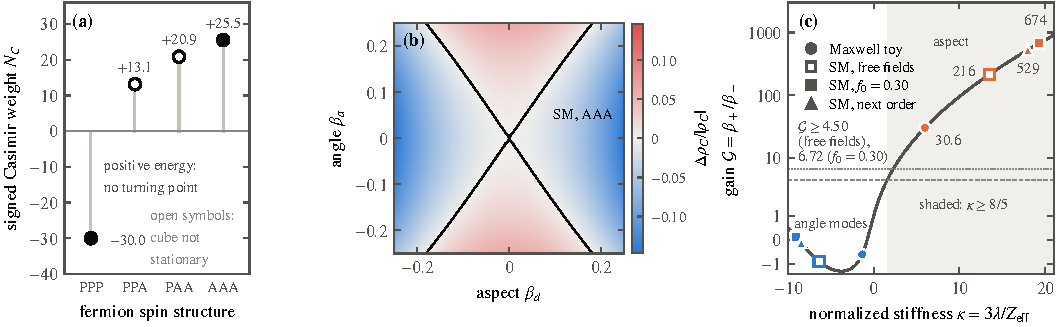
\includegraphics[width=\textwidth]{prd_casimir_shape}
\caption{Standard Model Casimir energy and its shape instability.
(a)~Signed Casimir weight $\NC$ of the high-energy Standard Model plus the static graviton on the cubic torus at trivial holonomy, for periodic (P) or antiperiodic (A) fermion cycles; filled: stationary cube.
(b)~Fractional change of the AAA Casimir energy density on the slice $G=\exp(2\beta_dX_d+2\beta_aX_{12})$; aspect deformations lower it, angle deformations raise it.
(c)~Gain of a linear shape mode versus normalized stiffness: Maxwell toy (circles), Standard Model with free fields (open squares), with $\fzm=0.30$ (filled squares) and at next order (triangles); shaded: $\kappa\geq8/5$ (Sec.~\ref{rep:shape}).}
\label{fig:rA-casimir-shape}
\end{figure}

\subsection{Flat gauge holonomies}
\label{rA:holonomy}

Flat gauge holonomies twist charged fields like spin structures, and charged fields give them a one-loop potential~\cite{Hosotani:1983xw}.
They enter Eq.~\eqref{eq:rA-imagesum} as additional twists, $\vartheta_i=Yg_i$ for a hypercharge holonomy $\bm g$ acting on a field of hypercharge $Y$, and $\vartheta_i=\pm k_i/3$ on (anti)triplets for an $SU(3)$ centre holonomy with integers $k_i$.
With periodic fermions the centre holonomies $\bm k=(1,1,1)$ and $(1,0,0)$ give $\NC=11.19$ and $0.56$, and the hypercharge holonomy $\bm g=g(1,1,1)$ gives $7.13$ at $g=3/2$ and at most $17.79$. %
So with periodic fermions an $SU(3)$ centre holonomy on all three cycles gives $\NC=+11.2$, and a hypercharge holonomy up to $+17.8$, and negative energy does not require antiperiodic fermions. %
These sectors break the cubic symmetry, and in the periodic case the energy decreases away from trivial holonomy.
For AAA the centre holonomies give $9.86$ and $22.74$, and $\NC$ along the hypercharge direction is maximal, $25.515$, at $g=0$. %
Trivial holonomy therefore maximizes $\NC$ along the hypercharge direction, and centre holonomies on one or three cycles lower it to $22.7$ and $9.9$, so the benchmark is stable against these deformations. %

\subsection{Sectors with 't~Hooft flux}
\label{rA:thooft}

In sectors with 't~Hooft flux the Standard Model fields are single valued only if a nontrivial $SU(3)$ or $SU(2)$ twist comes with a hypercharge flux $\Phi_Y$, and the smallest one is $|\Phi_Y|=2\pi$.
A constant hypercharge field strength with flux $\Phi_Y$ through a face of the cube has $F_{12}=\Phi_Y$ in coordinates of unit period, and its classical energy is
\begin{equation}
E_{\rm flux}=\frac{1}{2g_Y^2}\int d^3x\,\sqrt h\,h^{11}h^{22}F_{12}^2=\frac{\Phi_Y^2}{2g_Y^2L}\geq\frac{2\pi^2}{g_Y^2L}=\frac{100.7}{L}
\label{eq:rA-flux}
\end{equation}
at $g_Y(\mub)=0.443$. %
This is $2.36$ times the AAA Casimir energy $C/L$. %
A turn would need $\NC>2\pi^2/(g_Y^2\rAgam)=60$, whereas the Standard Model content gives at most $25.5$ for any flat twist, so these sectors cannot turn around. %

\subsection{Corrections to the field content}
\label{rA:content-corr}

Two smaller corrections concern the content.
The inflaton fluctuation is light at the turning point and adds $\tfrac12$ to $\NC$, which lowers the shape fossil of Sec.~\ref{rep:quantum-shape} by $2\%$ for free fields and by $3.5\%$ with the zero-mode energy of Sec.~\ref{rep:zeromodes}. %
Three right-handed neutrinos lighter than $2\pi/\Lb$ would add $0.70$, since three antiperiodic Weyl fermions contribute $3\times0.233673$. %
We keep the content of Eq.~\eqref{eq:rA-NCSM} and carry these effects in the error budgets of Secs.~\ref{rep:h-budget} and~\ref{rep:quantum-shape}.
Perturbative interactions of the nonzero modes correct $\NC$ by a relative amount of order $g^2/16\pi^2$.
The interactions of the constant modes are not perturbative at this size and are treated next.
